
\subsection{Coiled Tube and Sampling Bag Example} \label{sec:appA}
\subsubsection{CAC Coiled Tube} \label{A}
\begin{figure}[H]
    \begin{align*}
        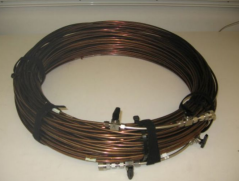
\includegraphics[width=0.6\linewidth]{appendix/img/cac-coil.png}
    \end{align*}
    \caption{CAC Coiled Tube.}
    \label{fig:A1}
\end{figure}

\subsubsection{Air Sampling Bag} \label{B}
\begin{figure}[H]
    \begin{align*}
        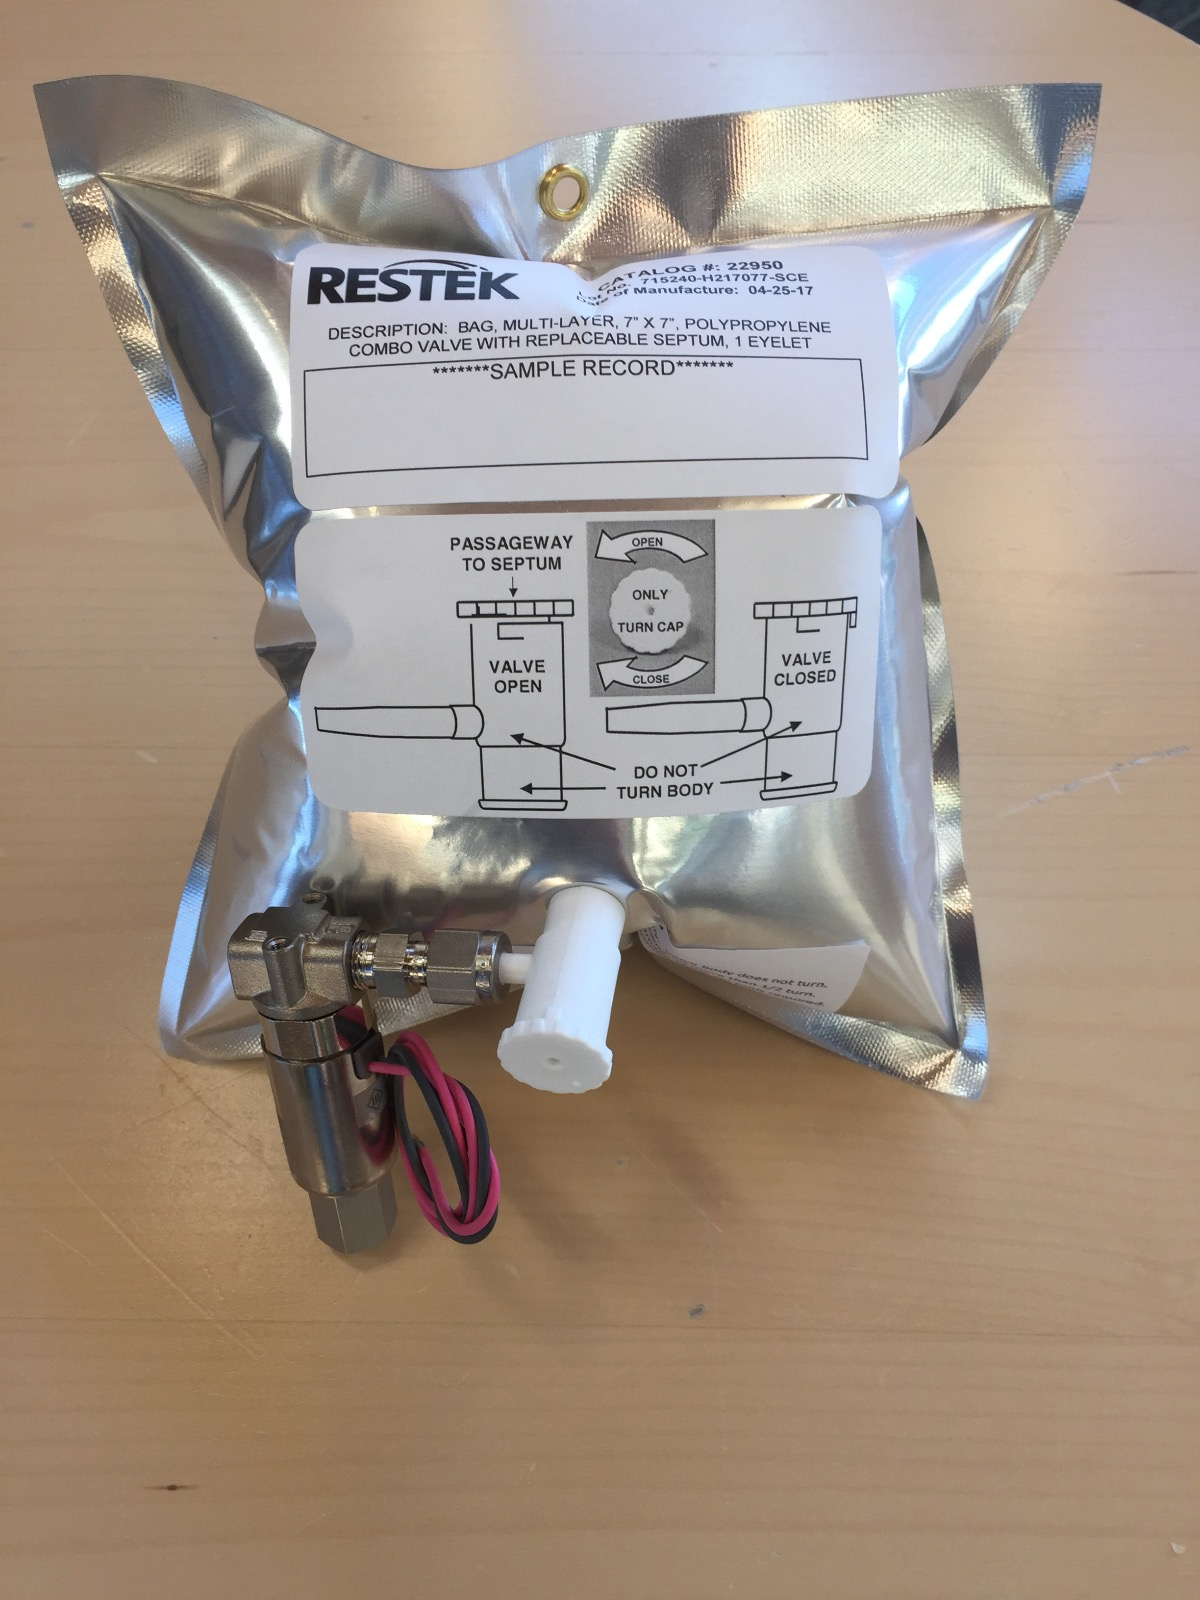
\includegraphics[height=0.4\linewidth]{appendix/img/Bag-we-use.jpg}
    \end{align*}
    \caption{Air Sampling Bag.}
    \label{fig:A2}
\end{figure}

\subsection{Dimensions of the sampling bag}
\label{dimensions-bags}

Table \ref{table:bags-dimensions} shows how the dimensions of the bags change according to the sampled volume. This data has been obtained by testing and has been taken into account in order to determine the maximum number of bags that can be filled inside the box.

\begin{table}[H]
\noindent\makebox[\columnwidth]{%
\scalebox{0.8}{
\begin{tabular}{|c|c|c|c|}
\hline
\textbf{Volume} & \textbf{Length (horizontal)}& \textbf{Height (vertical)} & \textbf{Width }\\ \hline
Empty & 26.4 cm & 28 cm & 0.5 cm \\ \hline
0.5 L & 26.4 cm & 27.5 cm & 1.5 cm \\ \hline
1 L & 26 cm & 27.5 cm & 2 cm \\ \hline
1.5 L & 25.5 cm & 26.5 cm & 4.5 cm \\ \hline
2 L & 25 cm & 25 cm & 5.5 cm \\ \hline
2.5 L & 24.5 cm & 23 cm & 7.5 cm \\ \hline
3 L & 24 cm & 22 cm & 10.5 cm \\ \hline
\end{tabular}}}
\caption{Dimensions of the Bags When Filled with Different Air Sample Volumes}
\label{table:bags-dimensions}
\end{table}